\documentclass[a4paper,12pt,oneside]{book}

\usepackage[DIV=15,headinclude=true,footinclude=false]{typearea}
\usepackage{fullpage} % Package to use full page
\usepackage{parskip} % Package to tweak paragraph skipping
\usepackage{tikz} % Package for drawing
\usepackage{amsmath}
\usepackage{hyperref}
\usepackage{listings}
\usepackage{color}
\usepackage{hyperref}
\usepackage[T1]{fontenc}
\usepackage[bitstream-charter]{mathdesign}
\renewcommand*\contentsname{Inhoud}

\usepackage{cclicenses}

%appendix usage
\usepackage[page]{appendix}

\usepackage{fancyvrb}
\usepackage{enumitem}
\usepackage{titlesec}
\usepackage[activate={true,nocompatibility},final,tracking=true,kerning=true,spacing=true,factor=1100,stretch=10,shrink=10]{microtype}

\hypersetup{
    colorlinks=true,
    linkcolor=blue,
    filecolor=magenta,      
    urlcolor=blue,
}

\definecolor{codegreen}{rgb}{0,0.6,0}
\definecolor{codegray}{rgb}{0.5,0.5,0.5}
\definecolor{codepurple}{rgb}{0.58,0,0.82}
\definecolor{backcolour}{rgb}{0.95,0.95,0.92}

\newcommand\PrevYear{%
   \advance\year by -1 \the\year\advance\year by 1}

\lstdefinestyle{mystyle}{
    backgroundcolor=\color{backcolour},   
    commentstyle=\color{codegreen},
    keywordstyle=\color{magenta},
    numberstyle=\tiny\color{codegray},
    stringstyle=\color{codepurple},
    basicstyle=\footnotesize,
    breakatwhitespace=false,         
    breaklines=true,                 
    captionpos=b,                    
    keepspaces=true,                 
    numbers=none,                    
    numbersep=5pt,                  
    showspaces=false,                
    showstringspaces=false,
    showtabs=false,                  
    tabsize=2,
    upquote=true
    frame=single
}
\let\oldlstinputlisting\lstinputlisting
% \lstinputlisting always have frame
\renewcommand{\lstinputlisting}[2][]{\oldlstinputlisting[frame=single]{#2}}

\lstset{basicstyle = \ttfamily,columns=fullflexible}

\titleformat{\chapter}{\normalfont\huge}{\thechapter.}{20pt}{\huge}[\titlerule]
\titleformat{\section}{\normalfont\Large}{\thesection.}{16pt}{\Large}
\titleformat{\subsection}{\normalfont\large}{\thesubsection.}{15pt}{\large}

\title{Programmeren voor dummies met Python \\ 

\includegraphics[width=0.2\textwidth]{img/by-nc.png}}
\author{Samuel Mok, docent Chemie, \href{s.mok@saxion.nl}{\textsf{s.mok@saxion.nl}}}
\date{Studiejaar \PrevYear/\the\year}



\end{center}
\begin{document}
\lstset{language=python}
\lstset{style=mystyle}

\maketitle
\tableofcontents

\chapter*{Introductie}
\addcontentsline{toc}{chapter}{Introductie}
In dit dictaat staat alle stof die je nodig hebt voor het vak Programmeren voor Dummies (2e jaar, kwartiel 4, opleiding Chemie). In dit vak wordt de programmeertaal Python gebruikt in combinatie met de software Pyzo om kennis te maken met programmeren. Het doel van het vak is dus niet om deelnemers binnen 4 weken vaardig te maken in programmeren, maar om in aanraking te komen met automatiseren en dataverwerken. 



Het vak is opgedeeld in 4 lessen.
\begin{itemize}
\item In de eerste les wordt de basis behandeld: hoe je code invoert en uitvoert, hoe je om input vraagt, en hoe je data op een simpele manier kan verwerken en kan laten zien. 
\item In de tweede les gaan we hier op verder en voegen we meer gereedschap toe om data te verwerken: loops, lijsten en functies. 
\item In de derde les leer je hoe je data uit een extern bestand kan ophalen en dit kan verwerken in bijvoorbeeld een grafiek. 
\item De laatste les is het uitvoeren van de eindopdracht van dit vak. 
\end{itemize}

Elke les bestaat uit een aantal verschillende onderwerpen. Per onderwerp zijn er een aantal oefeningen die je kunnen helpen met het begrijpen van de stof. Aan het einde van elk hoofdstuk staan een aantal opdrachten die testen of je de stof onder de knie hebt. De uitwerkingen van de opdrachten zijn beschikbaar. Houd er rekening mee dat als jouw antwoord net wat anders is, maar wel werkt, dit niet perse fout is. Er zijn vaak meerdere manieren om iets te programmeren.

Het dictaat is een onvolledige introductie tot Python. Python zelf heeft een uitgebreide tutorial (in het Engels) waar je alles kan vinden wat je nodig hebt, mocht het niet duidelijk worden uit het dictaat: \href{https://docs.python.org/3/tutorial/index.html}{https://docs.python.org/3/tutorial/index.html}. Handig om er naast te houden! Als je verder wil dan dit dictaat heeft de site datacamp.com erg goede tutorials en lesseries. Een aanrader is de volgende lesserie:
\href{https://www.datacamp.com/tracks/data-scientist-with-python}{Data scientist with Python}.

\textbf{Wat heb je nodig?}
\begin{itemize}
\item Een laptop met windows, MacOSX, of Linux
\item Dit dicaat
\item Een internetverbinding
\end{itemize}

Als je bovenstaande items hebt kan je starten aan dit vak. Voor het programmeren gebruiken we Pyzo, een gratis softwarepakket waar we in Python mee kunnen programmeren. Volg het onderstaande stappenplan om Pyzo te installeren.

Je kan ook met Python programmeren zonder iets te installeren. Je kan namelijk ook programmeren in je browser (Chrome, Firefox, wat dan ook). Je kan dat doen op de website \href{https://repl.it}{https://repl.it}. Maak een account aan, of log in met een bestaand account, en je kan gaan programmeren. Het is echter vaak handiger om Pyzo te installeren omdat je dan makkelijker kan werken met andere bestanden. Voor de eerste les maakt het niet veel uit.

LET OP: Het installeren van Pyzo duurt een tijdje, dus doe dat vantevoren! 

\textbf{Pyzo installeren}
\begin{itemize}
\item ga naar \href{http://www.pyzo.org/start.html}{http://www.pyzo.org/start.html}
\item Volg stap 1 t/m 3 (als stap 3 nog niet lukt: geen ramp!)
\end{itemize}

Als je Pyzo hebt geinstalleerd kan je aan de slag. Start het programma op. Je ziet als het goed is een scherm zoals in Fig.~\ref{fig:pyzokaal}.

\begin{figure}[h]
\begin{center}
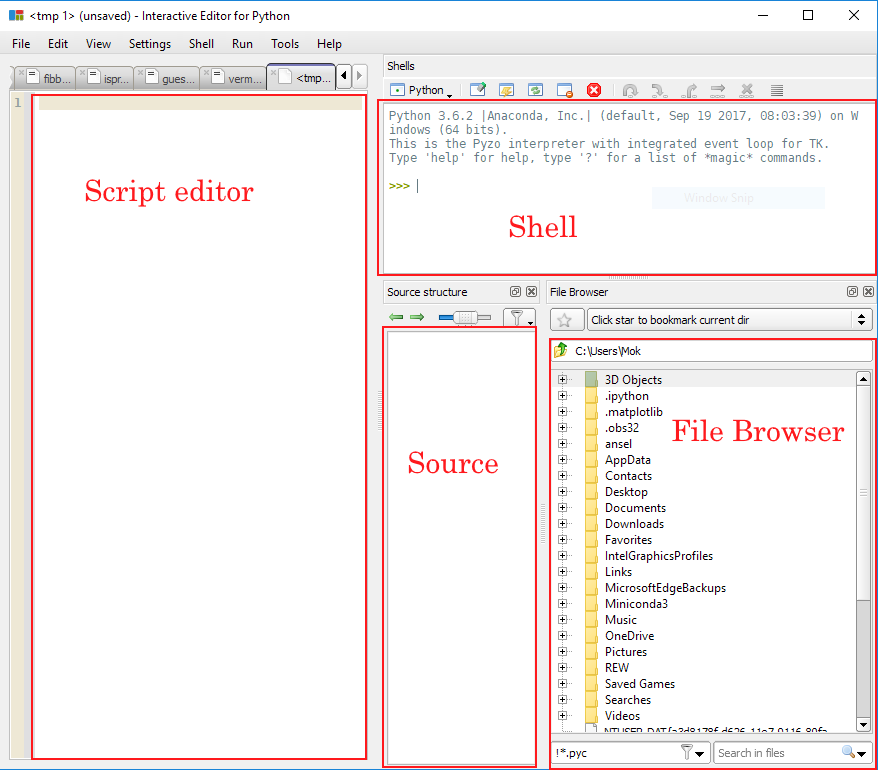
\includegraphics[width=0.6\textwidth]{img/pyzokaal.PNG}
\caption{\label{fig:pyzokaal} Pyzo zoals het eruit ziet als je het opstart. De rode text is later toegevoegd. }
\end{center}
\end{figure}

Dit is het hoofdscherm van Pyzo. Je ziet de volgende onderdelen:
\begin{itemize}
\item \textbf{Shell}: Dit is waar je output straks terecht komt, en waar je commando's in kan typen om uite voeren.
\item \textbf{Script Editor}: Dit is waar je langere code kan typen om op te slaan en te gaan draaien. Hierin werken we straks het meeste.
\item \textbf{Source}: Als je een groter, ingewikkeld programma hebt met meerdere bestanden zie je dat hier.
\item \textbf{File Browser}: Hier selecteer je in welke map je aan het werk bent.
\end{itemize}

In de Shell kan je dus code intypen om uit te voeren. Probeer het zelf: typ bijvoorbeeld in 5\texttt{+}8 en druk op enter. Wat je ook kan doen is je code in de Script Editor typen en dit script vervolgens uitvoeren. In les 1 gaan we hier mee bezig. In dit dictaat zullen voorbeelden worden gegeven van code, en dat ziet er als volgt uit:

\lstinputlisting{script/voorbeeld.py}

Je kan deze code kopieren in de Script Editor. Let wel op: Niet alles kopieert direct goed over. Let vooral op spaties, enters en tabs. Maak de code dus eerst netjes na het maken van de kopie.

Ga vervolgens naar Run -- Execute File om de code te draaien (of druk op CTRL-E). Als het goed is zie je dan de volgende output:
\begin{Verbatim}[frame=single]
>>> (executing file "<tmp 1>")
Hallo, chemicus!
13
Dit is het 0de nummer!
Dit is het 1de nummer!
Dit is het 2de nummer!
Dit is het 3de nummer!
Dit is het 4de nummer!
\end{Verbatim}

Als je een foutmelding krijgt heb je de code niet goed gekopieerd. Lees de foutmelding goed en zorg dat de code er exact hetzelfde uitziet als het voorbeeld! Als dit is gelukt ben je klaar om met het vak te beginnen.
\chapter{Les 1: Basisgebruik Python}
In de eerste les leren we op een simpele manier omgaan met Python. Onderwerpen die aan bod komen: rekenen met Python, het maken van eens script, datatypes, en if-statements. 

Officiele Python tutorial: \href{https://docs.python.org/3/tutorial/introduction.html}{Basis}

\section{Rekenen}
Voordat we met het "echte werk" beginnen gebruiken we eerst de Shell om rekenwerk uit te voeren. Je kan je rekenwerk gewoon intypen in de shell, en als je dan op enter drukt wordt het uitgevoerd. Let op: bij Python wordt een punt gebruikt ipv een komma voor waardes onder de 1. 

\textbf{A. Oefening rekenen}
\begin{enumerate}[label=\textbf{A.\arabic*}]
\item Reken de volgende vergelijking uit: $y = (2813*25) / (31091-34220*20)$
\item Een macht verheffen gaat zo: a ** b. Reken uit: 25 tot de macht 32. 
\item Bepaal de wortel van 382391. (als je niet weet hoe: kijk naar vorige opdracht!)
\end{enumerate}

Zoals je wellicht zal zien geeft Python antwoorden met veel decimalen. Deze kunnen we afronden met de de functie \textbf{round}. Functies worden in Python gebruikt voor bijna alle bewerkingen. Een functie bestaat uit een aanhef en argumenten, bij round bijvoorbeeld: round(a,b). A is het getal of berekening die je wil afronden, en b het aantal decimalen wat je wil zien. 

\textbf{B. Oefening afronden}
\begin{enumerate}[label=\textbf{B.\arabic*}]
\item Voer het volgende commando uit: $round((2813*25) / (31091-34220*20), 5)$. Verander vervolgens de laatste 5 in een ander getal. Wat gebeurt er?
\item Voer oefening A2 en A3 nog een keer uit, maar rond alles automatisch af op 2 cijfers achter de komma.
\end{enumerate}


Voor oefening B2 moest je nu weer opnieuw je formule intypen (of knippen/plakken). Dit kan natuurlijk makkelijker! Vanaf nu gebruiken we de Shell (bijna) niet meer, maar gaan we Scripts schrijven.


\section{Scripts \& datatypes}
Een script is een bestandje waar Python-code instaat die je kan uitvoeren. Zo hoef je niet iedere keer opnieuw dingen in te typen, en kan je overzichtelijker werken met variabelen en functies. Een script laat nooit iets zien in de Shell, behalve als je dat expliciet aangeeft. Dat gaat met de functie \textbf{print}. Functies worden later in meer detail uitgelegd. In de oefening hieronder oefenen we hiermee.

\textbf{C. Oefening scripts}
\begin{enumerate}[label=\textbf{C.\arabic*}]
\item Kopieer/plak de vergelijking van opdracht A.1 in het script (zie Fig.\ref{fig:pyzokaal}). Druk vervolgens op CTRL-E. Wat gebeurt er?
\item Typ de volgende code op de regel onder de vergelijking in je script: print(y). Voer uit. Wat zie je?
\item Verander print(y) in print(y+y). Voer uit. Verschijnt er wat je verwacht?
\item Typ nu: print(hallo). Voer uit.
\item Typ nu: print("hallo"). Voer uit.
\item Typ nu: print("hallo" + " allemaal"). Voer uit.
\item Typ nu: print("Het antwoord is " + y). Voer uit.
\item Typ nu: print("Het antwoord is " + str(y)). Voer uit.
\item Typ een \# aan het begin van een regel. Wat gebeurt er?
\end{enumerate}

Opdracht C.9 zorgt ervoor dat een regel uit je script niets doet. Het symbool \# markeert een regel code als commentaar. Python slaat deze regels over. Handig als je voor jezelf info in je script wil typen (bv waarom je iets hebt gedaan, etcetera). 

Zoals je ziet krijg je foutmeldingen bij opdrachten C.4 en C.7. Dit komt omdat Python alleen iets kan printen (=laten zien) als het een gedefinieerde variabele is. De variabele hallo bestaat niet, dus kan hij er niets mee bij opdracht C.4. \\
Bij opdracht C.5 heb je aanhalingstekens op hallo heengezet. Hiermee maak je aan Python duidelijk dat het je niet om een variabele gaat maar om een stuk text. Text heet in Python een \textit{string}. String betekent draad in het Engels, en het heet zo omdat een woord een draad (ketting) van individuele letters is. Een woord kan Python wel laten zien! \\
Als je meerdere woorden achter elkaar wil plakken kan je dat doen door de woorden bij elkaar op te tellen, zoals je ziet in opdracht C.6. Je kan geen getallen bij woorden optellen, zoals je ziet in opdracht C.7. Door het getal om te zetten naar text met de functie \textbf{str} kan het wel! \\
De verschillende soorten data noemen we \textit{datatypes}. De meest voorkomende: 

\textbf{Basisdatatypes}
\begin{itemize}
\item \textbf{Integer (int)} - een getal zonder cijfers achter de komma.
\item \textbf{Float (float)} - een getal met cijfers achter de komma.
\item \textbf{String (str)} - een stuk text; een aaneenschakeling van chars
\item \textbf{Boolean (bool)} - kan maar 2 waardes hebben: True of False. Kan worden vervangen door 1 en 0. 
\item \textbf{List} - een lijst met data. Gaan we later meer mee doen!
\end{itemize}

Voor ieder datatype is er een functie om een getal/text om te zetten in een bepaald datatype. Die functies staan tussen haakjes. Als je dus bijvoorbeeld y=\textbf{float}(21.3) intypt maak je variabele y aan met datatype float en waarde 21.3. Je hoeft in Python vaak niet zelf aan te geven wat voor soort datatype je waardes zijn, in de meeste gevallen wordt dat vanzelf goed gedetecteerd.

\section{Functies}

Een functie is een opdracht die je aanroept in Python. Je hebt hier vorige les al mee gewerkt: zo is bijvoorbeeld \textbf{print()} een voorbeeld van een functie. Een functie heeft  \textit{input} (ook wel argument(en) genoemd) en \textit{output}. De input komt tussen de haakjes en heeft een vorm die afhangt van de functie. Zo moet je bij de functie \textbf{print()}  altijd een string (text) invoeren om af te beelden. Als je getallen wil laten afbeelden zal Python deze automatisch proberen om te zetten naar text. Print heeft geen directe output die je kan opslaan: hij voert direct het commando uit.

Een voorbeeld van een functie met output is \textbf{random()}. Deze functie heeft geen input, alleen output. Als output geeft hij een komma-getal tussen de 0 en de 1. De output kan als volgt opslaan:
\begin{lstlisting}[frame=single]
y = random() 
\end{lstlisting}
y is nu dus een kommagetal tussen de 0 en de 1. 

Een voorbeeld van een functie met zowel argumenten als output is de functie \textbf{input()}. Als je het programma uitvoert zal deze functie een vraag stellen aan de gebruiker (de vraag is het argument van de functie), en het gegeven antwoord wordt opgeslagen als output. Dat kan bijvoorbeeld zo:
\begin{lstlisting}[frame=single]
getal = input("Welk geheel getal moet ik opslaan? ")
getal = int(getal)
\end{lstlisting}

Omdat het voor Python niet duidelijk is wat voor soort datatype het antwoord is moet je dan expliciet aangeven, zoals in de tweede regel is gedaan met de functie \textbf{int}. In de volgende les wordt uitgelegd hoe je je eigen functies kan maken.

\section{If-statements}
Officiele Python tutorial: \href{https://docs.python.org/3/tutorial/controlflow.html\#if-statements}{If-statements}

Nu weten we hoe een script werkt en wat voor gegevens we erin kunnen plaatsen. Dit kan je echter ook (bijna) allemaal gewoon met een simpele rekenmachine; we hebben hier dus niet zo veel aan. De kracht van programmeren ligt in het automatiseren van beslissingen op basis van gegevens. Het eerste hulpmiddel wat we hiervoor gebruik is de functie \textbf{if}. Deze functie doet iets als er iets waar of niet waar is. 

Een if-statement geef je in een specifieke vorm: \textbf{if} (conditie): \\
Bij (conditie) kan je invullen wat je je afvraagt, als je bijvoorbeeld wilt weten of 15 groter is dan y: \textbf{15 > y}. Als je iets wil doen als dat juist \textit{niet} waar is kan je de functie \textbf{else:} of \textbf{elif} gebruiken. \textbf{elif} staat voor else if, vertaald: anders als. Hier kan je dan nog een conditie toevoegen om te testen.

Een aantal voorbeelden van code vind je hieronder. Als je code kopieert als script in Pyzo zal je zien dat het foutmeldingen geeft: je moet de code exact overnemen, inclusie de spaties die voor sommige regels staan. Zonder deze spaties (in het Engels: indents) zal Python niet begrijpen wat je wil. Als je kopieert vanuit een PDF kan het zijn dat deze spaties niet meekomen. In het groen is commentaar opgenomen om uit te leggen wat iedere regel doet. 

\lstinputlisting{script/voorbeeldif2.py}
\lstinputlisting{script/voorbeeldif1.py}
\lstinputlisting{script/voorbeeldif3.py}

Je ziet nog twee nieuwe dingen in de voorbeelden staan. In het tweede voorbeeld wordt de functie \textbf{input} gebruikt. Bij input vraag je de gebruiker om... input. Als je de code draait krijg je de vraag/opdracht te zien die je als commando meegeeft aan de functie input. Alles wat de gebruiker intypt wordt opgeslagen als variabele, in dit geval als variabele x. Je ziet ook dat de functie \textbf{float} om de input heen staat, zodat de input van de gebruiker wordt opgeslagen als getal met cijfers achter de komma. Bij het gebruik van \textbf{input} moet je Python vertellen wat voor datatype je verwacht, anders kan je er niet goed verder mee werken. 

Het andere nieuwe wat je ziet is bij het laatste voorbeeld waar de functie \textbf{import} wordt gebruikt. Import zorgt ervoor dat je nieuwe functies aan je programma kan toevoegen. Hier is het pakket \textit{pandas} geimporteerd, een pakket die ondersteuning voor databases toevoegt aan Python. Hier gaan we later meer mee werken. 

\section{Opdrachten les 1: oefenen met input en if}
Bij de uitwerkingen van deze opdrachten zijn soms alternatieve manieren weergegeven die het iets beter of efficienter doen, met gebruik van functies of technieken die je (nog) niet hebt geleerd. Het is geen ramp als je dat niet allemaal snapt of het anders hebt gedaan: als je programma maar werkt! De docent kan alle antwoorden toelichten indien gewenst. 

\textbf{Les 1: Opdrachten}
\begin{enumerate}[label=\textbf{1.\arabic*}]
\item Maak een programma die vraagt om een letter en geef aan de gebruiker aan of dit een klinker of een medeklinker is. 
\item Maak een programma die vraagt om een golflengte in nm en geef aan: de frequentie van deze straling, welke kleur die straling heeft, en welke energie de straling heeft in J. Als de straling buiten het zichtbare gebied valt geef je dat ook aan. 
\item Maak een programma die om een getal vraagt met het commando \textbf{input} en geef aan de gebruiker aan of dit getal even of oneven is. Tip: gebruik de functie \textbf{\%} (deze heet modulo). Deze functie deelt het eerste getal door het tweede getal en geeft de rest terug. $10 \% 2$ geeft als antwoord 0, en $11 \% 2$ geeft als antwoord 1. 
\item Maak een programma die de gebruiker vraagt om 3 termen: $a, b, c$ van een polynoom van de vorm $ax^2 + bx + c$ . Geef het aantal nulpunten en de bijbehorende x-waardes terug.
\item Bonus: Modificeer de bovenstaande scripts met if-statements zodat ze een foutmelding geven als de gebruiker geen juiste invoer intypt. Denk bijvoorbeeld aan de situatie $a=0$ bij opgave 1.4. 
\end{enumerate}

\chapter{Les 2: Functies maken, Lijsten en Loops}
In deze les gaan we een flinke stap verder en gaan we dingen doen die lastig of tijdrovend zijn voor mensen, maar zo gepiept zijn als je het programmeert. De les begint met het schrijven van je eigen functies, gaat verder naar loops en het gebruik van lijst-datatypes. De les sluit af met het integreren van alle onderdelen tot nu toe.

\section{Zelf functies maken}
Officiele Python tutorial: \href{https://docs.python.org/3/tutorial/controlflow.html\#defining-functions}{Functions}

In de vorige les heb je gebruik gemaakt van functies, en geleerd dat ze input/argumenten hebben, en een output. Je kan ook functies toevoegen aan Python, sterker nog, alle functies die in Python zitten zijn door anderen gemaakt. Je kan ook met gemak extra functies toevoegen aan je script. De eerste is via \textbf{import}, zoals ook uitgelegd in paragraaf 1.4. De tweede is om je eigen functies te definieren. In deze paragraaf wordt uitgelegd hoe. We beginnen weer met een voorbeeld van een simpele functie die twee getallen bij elkaar optelt:

\lstinputlisting{script/voorbeeldFunctie.py}

De eerste regel van een functie bevat de term \textbf{def}, gevolgd door de naam van de functie, gevold door de argumenten die je wil gebruiken, en wordt afgesloten met een dubbele punt. In dit geval heet de functie dus \textbf{telop} met twee argumenten (twee getallen die opgeteld moeten worden).
In de regels eronder kan je wat gaan doen met de input; in dit geval tellen we ze bij elkaar op en slaan we het antwoord op in een nieuwe variabele \textit{output}. Een functie sluit je normaal af met de opdracht \textbf{return()}, waarbij je aangeeft wat de functie teruggeeft als antwoord. In dit geval dus de output (het opgetelde getal). Als je deze code in een script zet en uitvoert zal Python onthouden dat je een functie hebt gemaakt. Je kan hem nu gebruiken, bv in de shell als volgt:

\begin{lstlisting}[frame=single]
>>> telop(5,3)
8
\end{lstlisting}
Je kan ook een speciale waarde aan je output geven: \textit{None}. Dit herkent Python als lege waarde (dat is dus iets anders als 0). 
Het maken van functies is vooral handig als je bepaalde acties vaker uitvoert in een programma: dan hoef je niet iedere keer weer hetzelfde te gaan programmeren. Moet je bijvoorbeeld de nulpunten van een vergelijking willen weten kan je dat iedere keer helemaal uitschrijven, of een functie \textbf{vindNulpunt()} maken. Iets dergelijks kan je bijvoorbeeld doen voor opgave 1.4.

\textbf{A. Oefening functies} \\
Pak je script van opgave 1.4 er weer bij (waar je aan de hand van a, b, c de nulpunten van een polynoom bepaalde).
\begin{enumerate}[label=\textbf{A.\arabic*}]
\item Maak er nu een functie \textbf{vindNulpunt()} van. 
\\Deze heeft 3 argumenten (a,b,c). Er zijn 3 mogelijkheden voor de output: 0, 1, of 2 nulpunten. We gaan eerst de functie zo maken dat hij 1 output geeft, later breiden we het uit. Schrijf de functie op zo'n manier dat hij het nulpunt bepaalt bij D=0, het antwoord \textit{None} geeft als D < 0, en bij D > 0 alleen het antwoord met +wortel. Als je er moeite mee hebt: vraag hulp! De uitwerking staat in de bijlage. 
\end{enumerate}
Je merkt dat het onhandig is dat je maar 1 antwoord kan geven. Daarvoor is een oplossing: het gebruik van een lijst.

\section{Lijsten}
Officiele Python tutorial: \href{https://docs.python.org/3/tutorial/datastructures.html
}{Lijsten} \\
Een lijst is in Python een soort datatype. In plaats van een getal of een woord is het een verzameling van andere datatypen. Lijsten worden erg veel gebruikt.

Een lijst maak je door een set data gescheiden door komma's tussen blokhaken te zetten, bijvoorbeeld zo:
\begin{lstlisting}[frame=single]
>>> nummers = [1,2,3,4,5]
>>> nummers
[1, 2, 3, 4, 5]
\end{lstlisting}
Je kan de hele lijst dus aanroepen/printen door die variabele te gebruiken. Je kan ook een selectie maken uit de lijst of een individueel onderdeel van de lijst opvragen:
\begin{lstlisting}[frame=single]
>>> nummers[1]
2
>>> nummers[0]
1
>>> nummers[-1]
5
>>> nummers[-2]
4
\end{lstlisting}
Een lijst begint bij element of index 0. Het eerste ding dat je in de lijst stopt staat dus op plekje 0. Door nummers[0] aan te roepen vraag je dus het eerste element uit de lijst op. Bij het gebruik van een negatieve index vraag je getallen aan de achterkant van de lijst op: nummers[-1] is het laatste element uit de lijst, nummers[-2] het een-na-laatste, etcetera.

Het is ook mogelijk een deel van de lijst op te vragen. Dit heet een \textit{slice} (een stukje). Je krijg dan als antwoord een nieuwe lijst. Dit gaat met dubbele punten:

\begin{lstlisting}[frame=single]
>>> nummers[0:2]
[1,2]

>>> nummers[:2]
[1,2]

>>> nummers[2:]
[3,4,5]
\end{lstlisting}

Het werken met slices heeft dus twee argumenten: het begin en het eind, met een dubbele punt ertussen. Als je het eerste getal weglaat zal Python daarvoor zelf standaard 0 invullen, en als je het tweede getal weglaat zal Python daarvoor standaard het laatste element voor kiezen. 

Nu we weten hoe we met lijsten werken kunnen we onze functie vindNulpunt verder aanpassen zodat het 0, 1 of 2 nulpunten kan geven als antwoord.

\textbf{B. Oefening functie + lijst}
\begin{enumerate}[label=\textbf{B.\arabic*}]
\item Pas je functie vindNulpunt aan zodat het een lijst teruggeeft met de nulpunten. Bij geen nulpunten moet je nog steeds \textit{None} teruggeven.
\end{enumerate}

Er zijn een aantal standaardfuncties die je op een lijst kan uitvoeren. Een veelgebruikte functie is \textbf{lijst.append(data)}, die achteraan de lijst data toevoegt. De tegenhanger is \textbf{lijst.pop()} die het laatste element weer verwijdert en als output het verwijderde item geeft. Als je de eerste X elementen wil verwijderen kan je het commando \textbf{del lijst[:x]} gebruiken. 
Een voorbeeld:

\begin{lstlisting}[frame=single]
>>> lijst=[1,2,3]

>>> lijst
[1, 2, 3]

>>> lijst.append(4)

>>> lijst
[1, 2, 3, 4]

>>> lijst.pop()
4

>>> lijst
[1, 2, 3]
\end{lstlisting}

\section{Loops}
Officiele Python tutorial: \href{https://docs.python.org/3/tutorial/controlflow.html\#for-statements}{For-statements}\\
Loops (in het NL: lussen) zijn zeer belangrijke manieren om je programma vorm te geven. Ze vormen vaak de basis van veel programma's. Iedere keer dat je een lijst doorloopt of als je een functie wil uitvoeren op een set gegevens gebruik je een loop. De meest gebruikte vorm is een \textbf{for-loop}, en we besteden in dit onderdeel ook aandacht aan een \textbf{while-loop}. Daar beginnen we mee, want die is iets simpeler om te gebruiken.

Een \textbf{while-loop} is een commando die iets uitvoert zolang iets waar is. Een voorbeeld (draai de functie en kijk wat er gebeurt).

\lstinputlisting{script/voorbeeldwhile.py}

\textbf{C. Oefening while (antwoorden in bijlage)}
\begin{enumerate}[label=\textbf{C.\arabic*}]
\item Maak een while-loop die de getallen 1 t/m 10 afdrukt.
\item Maak een while-loop die een een getal \textit{a} tussen de 1 en de 100 vraagt en vervolgens 100-a uitrekent totdat het antwoord 0 of lager is, en aangeeft hoe vaak de loop heeft gedraaid.  
\end{enumerate}

Een andere vorm van loops zijn \textbf{for-loops}. Hier geef je een \textit{range} aan waar de loop tussen gaat lopen. Wederom is dit het meest makkelijk uit te leggen aan de hand van een (simpel) voorbeeld:
\lstinputlisting{script/voorbeeldFor.py}

en dit script geeft de volgende output:
\begin{lstlisting}[frame=single]
>>> (executing file "voorbeeldFor.py")
Dit is de 0de keer!
Dit is de 1de keer!
Dit is de 2de keer!
Dit is de 3de keer!
Dit is de 4de keer!
\end{lstlisting}

Een for-loop heeft 2 belangrijke componenten: de iterator (in dit geval i) en de range (bereik) van de loop. De iterator is een getal die telkens met een bepaalde stap wordt opgehoogd (standaard 1), en loopt dus met het bereik wat je aangeeft. Het bereik kan je invoeren zoals in het voorbeeld staat met de functie \textbf{range(nummerstart, nummereind, stapgrootte)}. In dit geval was het nummerstart niet ingevuld, en wordt er standaard 0 gekozen. nummereind is gelijk aan 5: de loop wordt dus 5x uitgevoerd. De stapgrootte is ook leeggelaten, en dan is het standaard gelijk aan 1. De iterator begint bij 0 en loopt dus 5x, waarmee bovenstaande output wordt gecreeerd. 

Het is ook mogelijk om loops binnen in loops te zetten, of if-statements in een loop te plaatsen, etcetera. Daar gaan we straks mee oefenen.


\textbf{D. Oefeningen for-loops (antwoorden in bijlage)}
\begin{enumerate}[label=\textbf{D.\arabic*}]
\item Maak een for-loop die de getallen van 1 t/m 40 bij elkaar optelt.
\item Maak een for-loop die de eerste 20 getallen van de tafel van 21 genereert in een lijst.
\item Gebruik for-loops om een driehoek van getallen te genereren. Vraag om het aantal rijen wat de gebruiker wil en maak vervolgens de structuur als volgt:\begin{lstlisting}1 
12 
123 
1234 
... etc. \end{lstlisting}
\end{enumerate}

\section{Opdrachten les 2: loops, functies en Lijsten}
\textbf{1. Priemgetallen}
\begin{enumerate}[label=\textbf{1.\alph*}]
\item Schrijf een script die een getal vraagt en vervolgens laat weten of dit een priemgetal is (dus alleen deelbaar door 1 en zichzelf) of niet. Tip: gebruik de modulo functie, \%. 
\item Pas dit script aan zodat het een functie is die je vanuit een ander programma kan aanroepen en een boolean (true/false) teruggeeft.
\item Pas de output van de functie aan: geef ook aan door welk getal het gedeeld kan worden als het geen priemgetal is. Geef dit mee als een integer. 
\item \textbf{Bonus:} Maak de functie zo efficient dat het getallen van 10 decimalen lang kan testen binnen enkele seconden, en laat het programma aangeven hoelang het erover deed om een antwoord te geven. Tip: gebruik het pakket \textit{datetime} en de functie \textbf{datetime.now()}. 
\end{enumerate}
\textbf{2. Gokken}
\begin{enumerate}[label=\textbf{2.\alph*}]
\item Raad het getal! Schrijf een programma die vraagt om een gok van de gebruiker. Geef aan of de gok juist is of niet en herhaal net zolang tot de gok goed is.
\item Laat het programma aangeven of het getal hoger/lager moet zijn.
\item Laat het programma een willekeurig getal tussen de 0 en de 100 genereren om te gokken. Gebruik uit het pakket \textit{random} de functie \textbf{random.random()}.
\item Geef aan het eind aan hoeveel pogingen er zijn gedaan en geef een mooi geformatteerde output. 
\end{enumerate}
\textbf{3. Fibbonacci-reeks}
\begin{enumerate}[label=\textbf{3.\alph*}]
\item Maak een programma die de eerste 10 getallen van de Fibbonacci-reeks weergeeft.
\item Maak een programma die de eerste X getallen van de Fibbonacci-reeks weergeeft, waarbij X wordt aangegeven door de gebruiker.
\item Maak een functie met X als argument die de eerste X Fibbonacci-getallen geeft in de vorm van een lijst.
\item \textbf{Bonus:} Pas de functie aan zodat je niet alleen de eerste X getallen kan opvragen maar begint op plek X en eindigt op plek Y. 
\end{enumerate}
\chapter{Les 3: Data importeren en verwerken}

Dit hoofdstuk zal ingaan op het importeren van gegevens uit bijvoorbeeld een excelbestand om daar een bewerking op los te laten / dingen mee te doen. Denk bijvoorbeeld aan het automatisch maken van een kalibratiecurve aan de hand van een reeks meetgegevens, en het daarmee uitrekenen van concentratie inclusief de juiste foutmarges.

Noot: Er zijn geen losse "eind"opdrachten voor deze les, gebruik de tijd voor de eindopdracht en het oefenen van de stof van afgelopen weken. 

Voor het importeren van data gebruiken we het pakket \textbf{pandas}. Dit staat voor \textbf{pan}el \textbf{da}ta\textbf{s}. Dit is een pakket die ervoor zorgt dat je een soort van database kan beheren in Python, zoals je wellicht mee bekend bent vanuit SQL. Pandas werkt samen met twee andere krachtige pakketten voor data-verwerking en plotten: \textbf{NumPy} en \textbf{Matplotlib}.\\ \textbf{NumPy} is een pakket waarmee multi-dimensionale arrays en matrices gemaakt kunnen worden en bevat ook fucties om hier berekeningen mee uit te voeren. \\
\textbf{Matplotlib} is een pakket waarmee je jouw data kan plotten in onder andere scatter plots, line plots en 3D plots.
\\ Omdat de pakketnamen vaak worden gebruikt worden ze vaak verkort geimporteerd in scripts, hieronder vind je de standaardmethode:
\begin{lstlisting}[frame=single]
import pandas as pd
import numpy as np
import matplotlib.pyplot as plt
\end{lstlisting}

Deze drie regels kan je bijna standaard in al je scripts zetten als je bezig gaat met data.

Dit hoofdstuk zal iets minder detail geven in de uitleg vergeleken met de vorige hoofdstukken: als het goed is ben je immers wat meer bekend met Python en programmeren. Bij ieder onderdeel worden linkjes gegeven met meer uitleg, voorbeelden, etcetera. Lees die ook door/gebruik die bij het doen van de opdrachten!

Als je meer hiervan wil weten is er online een heleboel hulp te vinden. Een zeer uitgebreide en goede tutorial vind je op datacamp, hier: \href{https://www.datacamp.com/tracks/data-scientist-with-python}{Data scientist with Python}.

\section{Pandas}
\href{http://pandas.pydata.org/pandas-docs/stable/10min.html}{Officiele pandas tutorial}\\
\href{http://pandas.pydata.org/Pandas_Cheat_Sheet.pdf}{pandas Cheat Sheet}

We beginnen met pandas. Met pandas kan je data in een soort tabel plaatsen, net zoals een lijst, maar dan met veel meer krachtige opties om de boel te rangschikken, verwerken, etcetera. Je kan dit direct invoeren in Python, maar vaak zal je bv een Excel-bestand hebben met je meetgegevens die je wil importeren. Als pandas een Excelbestand importeert zal hij het opslaan als een nieuw soort datatype: een \textbf{DataFrame}. 

Pandas gebruikt de eerste regel uit een Excel-bestand voor naamgeving. Jouw data wordt daarmee automatisch in logische rijen en kolommen gesorteerd. Het uitvoeren van statistiek gaat voornamelijk via het pakket \textbf{NumPy}, daar komen we later op terug. Als je data in een plot wil weergeven is daar het pakket \textbf{Matplotlib} voor. 
\\ Tip: Hou de tutorials open bij het maken van de opdrachten! Vanaf hier zal dit dictaat niet meer iedere stap uit gaan leggen (dan zou dit dictaat veel te groot worden): zoek dus zelf goed uit hoe je dingen aan zou moeten pakken.

\begin{figure}[h]
\begin{center}
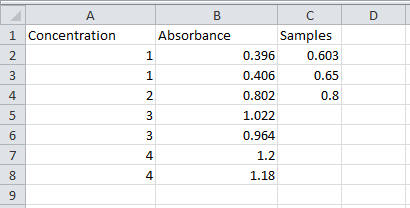
\includegraphics[width=0.6\textwidth]{img/excelscreen.PNG}
\caption{\label{fig:excel} De gebruikte excelsheet in dit voorbeeld. Opgeslagen als data.xlsx. }
\end{center}
\end{figure}

Een voorbeeld! We kunnen het Excelbestand in Fig \ref{fig:excel} importeren en weergeven met de volgende code:

\begin{lstlisting}[frame=single]
>>> data=pd.read_excel("data.xlsx")

>>> data
   Concentration   Absorbance  Samples
0               1       0.396    0.603
1               1       0.406    0.650
2               2       0.802    0.800
3               3       1.022      NaN
4               3       0.964      NaN
5               4       1.200      NaN
6               4       1.180      NaN
\end{lstlisting}

Een pandas DataFrame bestaat uit een verzameling van lijsten (daar heb je mee gewerkt in de vorige les). Elke lijst die je invoert is een rij en je kan elke rij een naam geven, wanneer je dat niet doet wordt deze automatisch genummerd te beginnen met 0.
Je kan ook zelf rechtstreeks data invoeren:

\begin{lstlisting}[frame=single]
>>> data=pd.DataFrame([[1, 2, 3], [4, 5, 6],[7, 8, 9]])

>>> data
   0  1  2
0  1  2  3
1  4  5  6
2  7  8  9

\end{lstlisting}
Wanneer je aan de kolomen een label wil geven doen je dat met "columns = []"

\begin{lstlisting}[frame=single]
>>> data = pd.DataFrame([[1,2,3],[4,5,6],[7,8,9]],columns = ["a", "b", "c"])

>>> data
   a  b  c
0  1  2  3
1  4  5  6
2  7  8  9

\end{lstlisting}
Een andere optie is een dictionary opgeven. \href{https://docs.python.org/2/tutorial/datastructures.html#dictionaries}{Officiele tutorial over dictionaries}.

\begin{lstlisting}[frame=single]
>>> data=pd.DataFrame({"a" : [1, 2, 3], "b" : [4, 5, 6], "c" : [7, 8, 9]})

>>> data
   a  b  c
0  1  4  7
1  2  5  8
2  3  6  9

\end{lstlisting}
Je ziet een aantal opvallende dingen. Zo heeft hij de 1e regel geimporteerd als namen van de kolommen (dat willen we graag!), is de eerste regel met data genummerd als regel 0 (net zoals met lijsten!) en zie je dat lege vakken worden gevuld met de text NaN. NaN staat voor "not a number" (=geen getal), en deze vakken zullen dus over worden geslagen bij berekeningen.
Een DataFrame kan meerdere typen data bevatten zoals, text, integers, floats en ook lege plekken, zoals je hierboven ook al hebt gezien. DataFrames zijn altijd 2D, dat wil zeggen dat ze altijd rijen en kolommen bevatten.

\section{Voorbeeld dataverwerking - Gamescores}
Noot: De complete tutorial vind je \href{https://www.dataquest.io/blog/pandas-python-tutorial/}{hier}, in het Engels, met plaatjes en extra uitleg. Hieronder een verkorte versie in het Nederlands. Voer de commando's zelf uit in Python om de output te zien. 

In dit voorbeeld gebruiken we een databestand die je hier kan downloaden: \href{http://www.sharecsv.com/s/3397aa3f9cf0cf20ae6c1428a32bfc07/ign.csv}{Klik!} 
Dit databestand bevat alle reviewscores die door website ign.com zijn toegekend. De dataset bevat verder nog meer info: welk platform de game op is gereviewed, in welk jaar, etcetera. Het is een .csv bestand, deze kan je ook importeren in Excel of SPSS. Met pandas kan je deze inlezen met de functie \textbf{read\_csv()}. Let op: het bestand wat je inleest moet in dezelfde directory staan als je pythonscript. Anders moet je het complete pad gebruiken. Daar moet je even opletten: gebruik dubbel slashes in het pad. In het voorbeeld zie je beide methodes:
\begin{lstlisting}[frame=single]
>>> import pandas as pd
>>> data = pd.read_csv("ign.csv") #lees bestand in
>>> data_complete_pad = pd.read_csv("C:\\Users\\Mok\\Downloads\\ign.csv") 
#gebruik hele pad als het niet goed werkt
\end{lstlisting}

We kunnen nu pandas vragen om een deel data netjes weer te geven. Voer de onderstaande code uit en je ziet als het goed is vanzelf wat de functies doen:
\begin{lstlisting}[frame=single]
>>> data.head(10) #eerste tien regels
>>> data.tail(7) #laatste 7 regels
>>> data.shape #aantal rijen en kolommen
(18625,11)
\end{lstlisting}

Het laatste commando geeft het aantal rijen en kolommen weer: er zijn dus meer dan 18000 reviews in dit bestand opgenomen, met 11 verschillende parameters per review. 

We kunnen ook wat statistiek doen:
\begin{lstlisting}[frame=single]
>>> data.mean()
>>> data.max()
>>> data.min()
>>> data.median()
>>> data.std()
>>> data.corr()
\end{lstlisting}

Je ziet dat pandas al deze functies op de hele dataset uitvoert. Je kan uiteraard ook individuele rijen of kolommen selecteren, of bijvoorbeeld kolom 1 t/m 5 van rij 1 t/m 100. Dit werkt eigenlijk hetzelfde als met lijsten, maar met iets andere commandos. Probeer het zelf (pas de cijfers aan en kijk wat er gebeurt!):
\begin{lstlisting}[frame=single]
>>> data.iloc[0:5,1]
>>> data.iloc[0:5,:]
>>> data.iloc[:,0:5]
>>> data.iloc[1,0:5]
>>> data.iloc[1:,:]
\end{lstlisting}

We kunnen zo dus ook de dataset opschonen. De eerste kolom bevat nutteloze info, dus laten we die weghalen:
\begin{lstlisting}[frame=single]
>>> data=data.iloc[:,1:] #eerste kolom weghalen
>>> data.head()  #checken of het goed is verwijderd
\end{lstlisting}

Dat werken met getallen is echter vaak niet handig. Nu moet je de hele tijd kijken welke rij ook alweer welke data had. Pandas maakt dat makkelijker voor je met labels. Je kan een naam koppelen aan een rij of kolom om zo makkelijk je data te selecteren. Dit zijn de namen die boven de kolommen staan in je data. Je kan dus bijvoorbeeld de volgende functies uitvoeren:
\begin{lstlisting}[frame=single]
>>> data.loc[0:5,"score"] #laat de kolom scores zien van rij 1 t/m 5
>>> data.loc[0:5,["score","release_year"]] 
#laat de score en uitgiftejaar zien van deze rijen
>>> data["score"] #laat de complete kolom score zien
\end{lstlisting}

Als we dus alleen geinteresseerd zijn in een deel van de info kunnen we dat selecteren. We kunnen ook filteren:
\begin{lstlisting}[frame=single]
>>> hoge_scores = data[data["score"]>7] 
#selecteer alle rijen waar de score hoger is dan 7
>>> hoge_scores.head(10)

>>> hoge_xbox_scores = hoge_scores[data["platform"] == "Xbox One"] 
#selecteer uit de lijst met hoge scores alle xbone games
>>> hoge_xbox_scores.head(10)
\end{lstlisting}

Het plotten van data kan ook. Je kan je bijvoorbeeld afvragen welk platform meer hoge scores krijgt: de PS4 of de XBOne?

\begin{lstlisting}[frame=single]
>>> import matplotlib.pyplot as plt
>>> ps4=data[data["platform"]=="PlayStation 4"] #alle ps4 data
>>> xbo=data[data["platform"]=="Xbox One"] #alle xbone data

>>> xbo["score"].plot(kind="hist") #plot alle xbox scores in een histogram
>>> plt.show() #laat de grafiek zien

>>> ps4["score"].plot(kind="hist") #plot alle ps4 scores in een histogram
>>> plt.show() #laat de grafiek zien
\end{lstlisting}

Als je de functies en hoe er mee om te gaan niet makkelijk kan onthouden: gebruik de cheat sheets die bovenaan het hoofdstuk staan. Dit zijn heldere overzichten van 1-2 A4 met alle belangrijke functies van pandas, numpy en matplotlib. Onthou: als je iets wil doen en je weet niet hoe: er is vast wel iemand die dat al een keer heeft geprobeerd, dus je kan in 9 van de 10 gevallen op internet gewoon het antwoord vinden. 

\textbf{A. Oefenen met pandas}
\begin{enumerate}[label=\textbf{A.\arabic*}]
\item Typ de dataset uit Fig~\ref{fig:excel} over in excel en sla op als data.xlsx. Importeer dit zoals uitgelegd in het hoofdstuk. Gebruik wat je hebt geleerd met pandas en voer een lineare regressie uit met de functie \textbf{linregress} uit het pakket \textit{scipy.stats}. \href{https://docs.scipy.org/doc/scipy/reference/generated/scipy.stats.linregress.html}{Hier de documentatie van linregress()}. 
\item Maak een plotje van de uitgevoerde lineare regressie (zie de link uit opdracht 3.1). Als het niet lukt: ga eerst verder met dit hoofdstuk, bij het deel matplotlib zal er meer info worden gegeven over het maken van plotjes.
\item Gebruik deze gegevens daarna om met behulp van een script de concentratie uit te rekenen van je samples. Als het niet lukt: ga googlen en je zal een heleboel uitgewerkte voorbeelden vinden! Als het niet lukt: ga eerst verder met dit hoofdstuk, bij het deel numpy zal meer info worden gegeven over het berekenen van data. 
\item BONUS: Pas je script aan zodat je het kan gebruiken met ieder willekeurig aantal meetpunten/samples. Maak er bijvoorbeeld een functie van die vanuit een XLSX of CSV direct de concentraties teruggeeft. De vorm van de data blijft altijd hetzelfde: eerst concentratie, dan absorbance, dan de samplewaardes.
\item Meer oefeningen vind je \href{https://github.com/ajcr/100-pandas-puzzles}{hier!}
\end{enumerate}

\section{Numpy}
\href{https://docs.scipy.org/doc/numpy/user/quickstart.html}{Officiele numpy tutorial}\\
\href{https://s3.amazonaws.com/assets.datacamp.com/blog_assets/Numpy_Python_Cheat_Sheet.pdf}{numpy Cheat Sheet}\\
\href{http://cs231n.github.io/python-numpy-tutorial/#numpy}{extra numpy-tutorial}\\
Numpy is een pakket waarmee je numpy-arrays kan maken en bewerken. Numpy-arrays zijn een speciaal soort lijsten, met veel ingebouwde functies. Als je wat geavanceerdere bewerkingen wil uitvoeren is dit pakket onmisbaar. Een numpy-array is direct te vergelijken met een matrix (zoals je bij wiskunde/lineaire algebra hebt gehad).
\\De belangrijkste verschillen tussen NumPy-arrays en Pandas-DataFrames zijn dat in NumPy-array maar \'e\'en type data kan staan, in tegenstelling tot Pandas-DataFrames waarbij je meerder typen data kan combineren. Waar Pandas-Dataframe altijd 2D is kunnen Numpy arrays veel meer dimensies hebben.

Het aanmaken van numpy arrays is simpel. Voer de onderstaande code uit en je ziet vanzelf wat er gebeurt:
\begin{lstlisting}[frame=single]
>>> import numpy as np
>>> a = np.array([1,2,3])
>>> a
>>> a[0]
>>> a[0:2]
>>> b = np.array([[1,2,3],[4,5,6]])
>>> b[0]
>>> b[0,0]
>>> b
\end{lstlisting}

In plaats van alle individuele getallen in de matrix te zetten zijn er ook functies om ze snel te maken. Probeer onderstaande code en kijk wat het maakt (en verander de getalletjes!):
\begin{lstlisting}[frame=single]
>>> a = np.zeros((5,5))
>>> b = np.ones((3,2))
>>> c = np.full((2,5),9)
>>> d = np.eye(5)
>>> e = np.random.random((4,3))
>>> f = np.arange(1,10,0.1)
\end{lstlisting}

Het opvragen van data uit een np-array gaat op dezelfde manier als uit lijsten: met slices.
Wanneer je een np-array sliced geeft het cijfer voor de komma het rijnummer aan en het cijfer na de komma de kolom. 
Probeer dit zelf ook uit met arrays met verschillende dimensies. Vergeet niet dat in python de nummering met 0 begint. Dus de eerste rij heeft rijnummer 0, de 2e rijnummer 1, etc.

\begin{lstlisting}[frame=single]
>>> a = np.random.random((4,4))

>>> a
array([[ 0.45423941,  0.02449346,  0.28748383,  0.86696254],
       [ 0.84538737,  0.88094837,  0.82634451,  0.46029926],
       [ 0.6649267 ,  0.23539764,  0.24480059,  0.40225708],
       [ 0.69317471,  0.70946337,  0.23112397,  0.45701743]])

>>> a[0,:]
array([ 0.45423941,  0.02449346,  0.28748383,  0.86696254])

>>> a[:,0]
array([ 0.45423941,  0.84538737,  0.6649267 ,  0.69317471])

>>> a[3,3]
0.45701742997293382

>>> a[0:2,2:4]
array([[ 0.28748383,  0.86696254],
       [ 0.82634451,  0.46029926]])
       
\end{lstlisting}

Net zoals in een pandas-array kan je ook data selecteren met behulp van voorwaarden:
\begin{lstlisting}[frame=single]
>>> a = np.array([1,2,3,4,5,6,7,8,9,10])
>>> b = a[(a>4)] #b=alle getallen groter dan 4 uit a
>>> c = a[(a%2==0)] #c=alleen even getallen uit a
\end{lstlisting}

we kunnen ook rekenen met arrays alsof het matrices zijn:
\begin{lstlisting}[frame=single]
>>> a = np.array([1,2,3,4,5,6,7,8,9,10])
>>> c=a*2
>>> b = np.full((1,10),3)
>>> d=a*b
>>> e=a/b
\end{lstlisting}

Kijk in de tutorials en de cheat-sheet voor meer handige en nuttige functies van numpy.

\textbf{B. Oefenen met numpy}
\begin{enumerate}[label=\textbf{B.\arabic*}]
\item Maak een functie die alle even getallen in een 1 bij X matrix negatief maakt.
\item Maak zelf een functie die uit een random matrix van 100x100 het hoogste getal teruggeeft. Gebruik de functie np.max om je antwoord te controleren.
\item als je meer wil oefenen, kijk dan \href{https://www.machinelearningplus.com/python/101-numpy-exercises-python/}{hier!}
\end{enumerate}

\section{Matplotlib}
\href{https://matplotlib.org/users/pyplot_tutorial.html}{Officiele matplotlib tutorial}\\
\href{https://s3.amazonaws.com/assets.datacamp.com/blog_assets/Python_Matplotlib_Cheat_Sheet.pdf}{matplotlib Cheat Sheet}

Matplotlib is een pakket om plotjes te maken. Om te beginnen heb je uiteraard eerst data nodig, deze data kan je importeren met pandas en bewerken met numpy, zoals je in de vorige paragrafen hebt geleerd.
Online is veel data verkrijgbaar een goede bron om mee te oefenen is de data van het cbs. 
\href{https://opendata.cbs.nl/#/CBS/nl/dataset/37221/table?dl=14447}{De data die gebruikt wordt voor de volgende voorbeelden kan je hier vinden.}
Stap 1 is het importeren van de data:

\begin{lstlisting}[frame=single]
>>> pd_uitstoot = pd.read_csv("C:/Emissies_naar_lucht_op_Nederlands_grondgebied__totalen_11112018_170037.csv")

>>> pd_uitstoot.head()
  Emissies naar lucht op Nederlands grondgebied; totalen
0                                                NaN    
1                                   ;"";"";"Bronnen"    
2  Onderwerp;"Perioden";"";"Totaal Stationaire en...    
3  CO2;"1990";"mln kg";"170410";"22080";"7550";"2...    
4  CO2;"1995";"mln kg";"180590";"17230";"7750";"2... 
\end{lstlisting}

Zoals je kan zien is het niet helemaal goed gegaan, dus zullen we eerst de data wat moeten opschonen.

\begin{lstlisting}[frame=single]
>>> pd_uitstoot = pd.read_csv("C:/Emissies_naar_lucht_op_Nederlands_grondgebied__totalen_11112018_170037.csv", skiprows = 3, sep = ";")

>>> pd_uitstoot.head()
  Onderwerp Perioden Unnamed: 2  Totaal Stationaire en mobiele bronnen  \
0       CO2     1990     mln kg                               170410.0   
1       CO2     1995     mln kg                               180590.0   
2       CO2     2000     mln kg                               182610.0   
3       CO2     2005     mln kg                               190780.0   
4       CO2     2010     mln kg                               198940.0   

   20-21 Chemie en farmaceutische industrie  24 Basismetaalindustrie  \
0                                   22080.0                   7550.0   
1                                   17230.0                   7750.0   
2                                   16470.0                   6360.0   
3                                   16280.0                   7240.0   
4                                   18200.0                   6890.0   

   Particulier huishouden  01 Landbouw (stationaire bronnen)  Vervoer  \
0                 22350.0                             7750.0  29860.0   
1                 25030.0                             8260.0  31710.0   
2                 22320.0                             7500.0  35660.0   
3                 21710.0                             7440.0  37810.0   
4                 25350.0                            10190.0  37780.0   

   Railverkeer  Wegverkeer  Scheepvaart  Luchtvaart  
0         90.0     23980.0       5470.0       320.0  
1         90.0     25570.0       5600.0       450.0  
2        110.0     28290.0       6640.0       610.0  
3        110.0     29910.0       7110.0       680.0  
4        110.0     29960.0       7040.0       670.0  

\end{lstlisting}

Nu we de data in een pandas DataFrame hebben staan kunnen we de data opschonen. De laatste rij bevat een hoop NaN. Met df.dropna() worden alle rijen waar NA (not available) of NaN (not a number) staat verwijderd.

\begin{lstlisting}[frame=single]
>>> pd_uitstoot = pd_uitstoot.dropna()
\end{lstlisting}

Wanneer we de uitstoot van railverkeer en luchtvaart met elkaar willen vergelijken kunnen we deze op verschillende manieren in een plot weergeven. Hieronder een voorbeeld:

\begin{lstlisting}[frame=single]
>>> pd_uitstoot["Perioden"][8] = 2017

>>> x = pd_uitstoot["Perioden"]

>>> y = pd_uitstoot["Railverkeer"]

>>> plt.scatter(x, y, label = "Railverkeer")
<matplotlib.collections.PathCollection object at 0x0000000004F36C88>

>>> z = pd_uitstoot["Luchtvaart"]

>>> plt.scatter(x, z, label = "Luchtvaart")
<matplotlib.collections.PathCollection object at 0x0000000004F5E1D0>
>>> plt.show()
\end{lstlisting}

Het plotje komt er dan uit te zien zoals in Fig. ~\ref{fig:matplotlib_scatter_1}

\begin{figure}[h]
\begin{center}
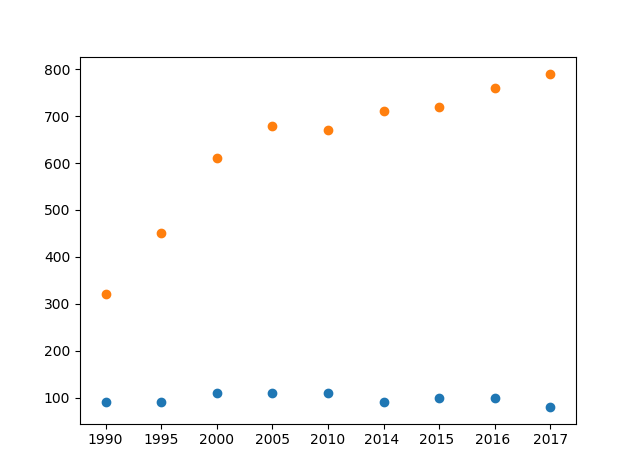
\includegraphics[width=0.6\textwidth]{img/matplotlib_scatter_1.png}
\caption{\label{fig:matplotlib_scatter_1} Scatterplot van de uitstoot railverkeer en luchtverkeer per jaar}
\end{center}
\end{figure}

Zonder labels en legenda is deze plot niet compleet, dus laten we die toevoegen!

\begin{lstlisting}[frame=single]
>>> plt.xlabel("Jaar")
Text(0.5,0,'Jaar')

>>> plt.ylabel("mln kg")
Text(0,0.5,'mln kg')

>>> plt.legend()
<matplotlib.legend.Legend object at 0x00000000086C5BE0>

>>> plt.show()

\end{lstlisting}

Met labels komt het de grafiek er dan uit te zien als Fig.~\ref{fig:matplotlib_scatter_2}.

\begin{figure}[h]
\begin{center}
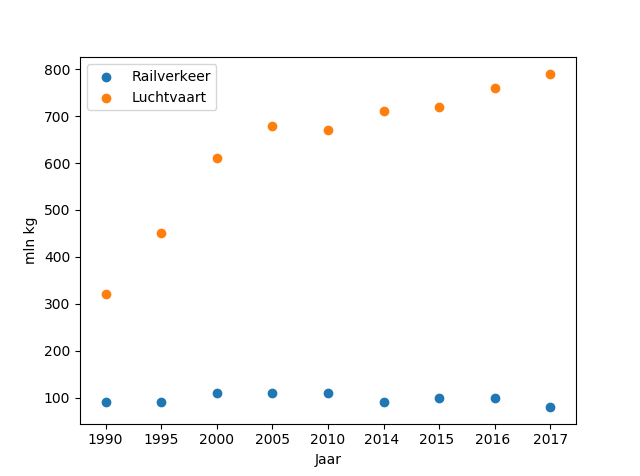
\includegraphics[width=0.6\textwidth]{img/matplotlib_scatter_2.png}
\caption{\label{fig:matplotlib_scatter_2} Scatterplot van de uitstoot railverkeer en luchtverkeer per jaar met labels}
\end{center}
\end{figure}

\textbf{C. Oefenen met Matplotlib}

\begin{enumerate}[label=\textbf{C.\arabic*}]
\item Maak een plot van de ign.csv data met behulp van matplotlib. Kies zelf wat je wil plotten. Selecteer de data met behulp van pandas, en maak de plot mooi met matplotlib. 
\item Meer oefeningen vind je \href{https://www.w3resource.com/graphics/matplotlib/}{hier!}
\end{enumerate}



\chapter{Les 4: Eindopdracht}

De details van de eindopdracht staan op Blackboard. Inhoudelijk wordt er hier een voorzet gegeven.

Het doel is om een script te schrijven die een bewerking voor je automatiseert. Zo kan je bijvoorbeeld denken aan een simpele UV-VIS meting. Als data heb je een bestand met concentraties, bijbehorende extincties en de extincties van onbekende samples, net zoals in les 3 als voorbeeld is gebruikt. Je kan dan een script maken in Python die een dergelijk excel-bestand inleest, een kalibratiecurve maakt, en met de gegevens de concentraties van de samples berekent inclusies foutmarges. 

Er zijn natuurlijk oneindig veel bewerkingen die je kan doen en die je dus ook kan automatiseren. Maak een keus en schrijf je script. De belangrijkste tip: gebruik google! Zoek (in het Engels) wat je wil weten, en de kans is groot dat iemand het al eens heeft gedaan. Het is niet noodzakelijk dat je iedere regel code zelf hebt bedacht. Het is uiteraard geen enkel probleem om code van anderen over te nemen, als het eindproduct maar iets is wat je persoonlijk hebt gemaakt en kan gebruiken. 
De stof van les 3 (pandas, numpy, matplotlib) zijn essentieel voor het goed uitwerken van deze opdracht.

Het doel van deze opdracht is dus iets automatiseren wat je anders handmatig deed, en niet zozeer om te laten zien dat je een top-programmeur bent. De diepgang van de code zal dus per persoon verschillen: de een zal een ingewikkelder programma schrijven dan de ander. Dat is geen probleem, als je maar laat zien dat je een bewerking kan automatiseren.

Dit is ook de reden dat iedereen een persoonlijke opdracht krijgt. Op Blackboard staat er informatie over hoe dit te werk gaat.

Het eindproduct van deze opdracht is de code die je hebt gemaakt, de input die je gebruikt, en de output die het genereert, en daarbij een  beschrijving en toelichting. Lever het aan als .docx of .pdf bestand in Blackboard. Zorg ervoor dat je ook data mee levert zodat de docent de werking van het programma kan controleren.  
\begin{appendices}
\chapter{Antwoorden/uitwerkingen opdrachten}
Let op: deze manier van uitwerken hoeft niet perse de beste manier te zijn, met programmeren kan je immers op heel veel manieren een probleem oplossen. Het gaat niet om hoe je het doet, maar of je begrijpt wat er gebeurt. Werkende code is belangrijker dan mooie code!

\section{Les 1}
\lstinputlisting{script/uitwerking1.1.py}
\lstinputlisting{script/uitwerking1.2.py}
\lstinputlisting{script/uitwerking1.3.py}
\lstinputlisting{script/uitwerking1.4.py}

\section{Les 2}
\textbf{Oefeningen}
\lstinputlisting{script/vindnulpunt.py}
\lstinputlisting{script/uitwerkingWhile.py}
\lstinputlisting{script/uitwerkingOefenFor.py}

\textbf{1. Priemgetallen}
\lstinputlisting{script/isprime.py}

\textbf{2. Gokken}
\lstinputlisting{script/guess.py}

\textbf{3. Fibbonaci}
\lstinputlisting{script/fibbonaci.py}

\section{Les 3}
\textbf{A. Oefenen met pandas}
\lstinputlisting{script/pandas_uitwerking.py}
\textbf{B. Oefenen met numpy}
\lstinputlisting{script/numpy_uitwerking.py}

\end{appendices}




\end{document}